%\subsection{Bleichenbacher's Attack.}
%One of the most important attacks in the TLS history is the million's message attack, published by Daniel Bleichenbacher at Crypto 1998~\cite{Bleichenbacher}. The attack targets the RSA \PKCS encryption scheme, which is used in the TLS protocol to encrypt a so called \pms. The \pms a 48 byte value sent by the client to the server, encrypted using server's public key. Based on the \pms, both peers can derive \textit{all} keys needed for secure communication.
%
%Essentially, Bleichenbacher's attack is an adaptive chosen-ciphertext attack or, more commonly known, a padding oracle attack. The attack assumes existence of an oracle that responds with "valid" or "invalid" according to the \PKCS validity of the decrypted message. The attacker exploits such an oracle as follows. It starts the attack with an RSA ciphertext (containing an encrypted \pms), which he obtained for example by observing the traffic between the client and the server. The attacker then modifies this ciphertext, sends it to the server, and observes the ciphertext validity. With each valid ciphertext, the attacker learns several plaintext bits. At the end, by sending several thousands of messages the attacker can decrypt the whole \pms, and thereby decrypt a TLS session.

In the following, $a||b$ denotes concatenation of strings $a$ and
$b$. $a{[i]}$ references the $i$-th byte in $a$.
$(N,e)$ denotes an RSA public key, where $N$ has byte-length
$\ell$ ($|N|=\ell$) and $e$ is the public exponent. The corresponding
secret exponent is $d = 1/e \bmod \phi(N)$.

\subsection{\PKCS encryption padding}
\label{sec:PKCSdescr}

Our attacks rely on the structure of RSA \PKCS padding.  Although there are newer versions of the PKCS standard,
for example RSA PKCS\#1 v2.0 which implements OAEP, SSL/TLS uses \PKCS.
The basic task of the \PKCS encryption padding scheme~\cite{rfc2313}
is to randomize encryptions by prepending a random padding string $PS$
to a message $k$ (typically a symmetric session key) before applying
RSA encryption:

\begin{enumerate} 
	\item The plaintext message is $k$. The encrypter generates a random byte
	string $PS$, where $|PS| \geq 8$, $|PS|=\ell-3-|k|$, and $\hex{00} \not \in \{PS{[1]}, \ldots,PS{[|PS|]}\}$. 
	\item The encryption block is $m = 00||02||PS||00||k$. 
	\item The ciphertext is computed as $c = m^e \bmod N$. 
\end{enumerate} 

To decrypt such a ciphertext, the decrypter first computes $m = c^d
\bmod N$.  Then it checks whether the decrypted message $m$ is
correctly formatted as a \PKCS-encoded message. We say that the
ciphertext $c$ and the decrypted message bytes $m{[1]} || m{[2]} || ... ||
m{[\ell]}$ are \PKCSconform if:
\begin{equation*} 
	\begin{split} 
		m{[1]}||m{[2]} \text{ } = &\text{ } \hex{00} || \hex{02}\\
		\hex{00} \text{ } \not \in &\text{ } \{m{[3]}, \ldots,m{[10]}\}\\ 
	\end{split}
\end{equation*} 
If this condition holds, the decrypter searches for the first value
$i>10$ such that $m{[i]}=0x00$. Then, it extracts $k =
m{[i+1]}||\ldots||m{[\ell]}$. Otherwise, the ciphertext is rejected.

In SSLv3 and TLS, RSA \PKCS is used to encapsulate the
\pms exchanged during the
handshake~\cite{rfc5246}. Thus, $k$ is interpreted as the
\pms.  In SSLv2, RSA \PKCS is used for
encapsulation of an equivalent key denoted the \texttt{master\_key}.


\subsection{SSL and TLS}
The first incarnation of the TLS protocol was the SSL (Secure Socket
Layer) protocol, which was designed by Netscape in the 90s. The first two
versions of SSL were immediately found to be vulnerable to trivial
attacks~\cite{ProhibitingSSLv2,WagnerSchneier:SSLAnalysis:96} which 
were fixed in SSLv3~\cite{SSLv3}.  Later versions of
the standard were renamed TLS, and share a similar structure to SSLv3.
The current version of the protocol is TLS 1.2; TLS 1.3 is currently
under development.

An SSL/TLS protocol flow consists of two phases: handshake and
application data exchange. In the first phase, the communicating
parties agree on cryptographic algorithms and establish shared
keys. In the second phase, these keys are used to protect the
confidentiality and authenticity of the transmitted application data.

The handshake protocol was fundamentally redesigned in the \sslthree
version. This new handshake protocol was then used in later TLS
versions up to TLS 1.2. In the following, we describe the RSA-based
handshake protocols used in TLS and \ssltwo, and highlight their
differences.

%\paragraph{Cipher Suites.}
%The SSL/TLS protocol flow uses different cryptographic algorithms for data encryption, signature computation, or HMAC generation. A set of cryptographic algorithms used during a protocol flow is summarized in a cipher suite. For example, a \texttt{TLS\_RSA\_WITH\_AES\_128\_CBC\_SHA} cipher suite denotes that the established connection uses RSA \PKCS encryption scheme to exchange keys, AES-128 in CBC mode for data encryption, and SHA-1 for HMAC computation. 

%The TLS protocol supports further cipher suites with Diffie-Hellman key exchange algorithms or pre-hared keys. However, in the following we will concentrate on the description of TLS-RSA handshakes since these are relevant to our attacks. %We also omit description of client authentication.


%This subsection briefly surveys the general workings of SSLv2 - interested readers are encouraged to read the full protocol description \cite{SSLv2}. We note that the description was apparently written during the early stages of the standardization efforts of the Internet suite of protocols, and accordingly, is much less rigorous and formally defined than more modern RFCs. For lack of a better term, we shall henceforth refer to this document as the SSLv2 standard, or simply as the standard, although the term could reasonably be considered inadequate due to the lack of rigorousity.

\paragraph{The \ssltwo handshake protocol.}
\label{sec:ssl2}
The \ssltwo protocol description~\cite{SSLv2}  is much less formally specified than modern RFCs. Figure~\ref{fig:ssl-handshake} depicts an \ssltwo handshake.
%
%\ifext
% Juraj: we can rather remove the TLS protocol figure...everybody knows TLS or can easily find a nice protocol description
\begin{figure}
	%\centering 
	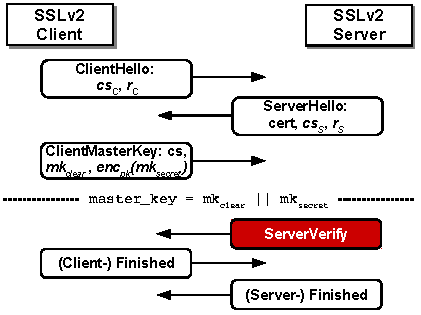
\includegraphics[width=\linewidth]{img/ssl-handshake} 
	\caption{\textbf{\ssltwo handshake.} The server responds with a \texttt{ServerVerify} message directly after receiving an RSA-\PKCS ciphertext contained in \texttt{ClientMasterKey}. This protocol feature enables our attack.\looseness=-1}
	\label{fig:ssl-handshake}
\end{figure}
%\fi
%
A client initiates an \ssltwo handshake by sending a
\texttt{ClientHello} message, which includes a list of cipher
suites $cs_c$ supported by the client and a client nonce $r_c$,
termed \texttt{challenge}.
The server responds with a \texttt{ServerHello} message, which
contains a list of cipher suites $cs_s$ supported by the server,
the server certificate, and a server nonce $r_s$, termed
$\texttt{connection\_ID}$.

The client responds with a \texttt{ClientMasterKey} message, which
specifies a cipher suite supported by both peers and key data
used for constructing a \texttt{master\_key}. In order to support
\textit{export} cipher suites with 40-bit security (e.g.,
\texttt{SSL\_RC2\_128\_CBC\_EXPORT40\_WITH\_MD5}), the key data is
divided into two parts:
\begin{itemize}
	\item $mk_{clear}$: A portion of the \texttt{master\_key} sent in the \texttt{ClientMasterKey} message as plaintext (termed \texttt{clear\_key\_data} in the \ssltwo standard).
	\item $mk_{secret}$: A secret portion of the
          \texttt{master\_key}, encrypted with RSA \PKCS (termed \texttt{secret\_key\_data}). 
\end{itemize}
The resulting \texttt{master\_key} $mk$ is constructed by
concatenating these two keys: $mk = mk_{clear} || mk_{secret}$. For
40-bit export cipher suites, $mk_{secret}$ is five bytes in length.
For non-export cipher suites, the whole \texttt{master\_key} is
encrypted, and the length of $mk_{clear}$ is zero.

The client and server can then compute session keys from the reconstructed \texttt{master\_key} $mk$:

\begin{center}
\begin{math}
	\texttt{server\_write\_key} = MD5(mk || ``0" || r_c || r_s) \linebreak	
	\texttt{client\_write\_key} = MD5(mk || ``1" || r_c || r_s)
\end{math}
\end{center}

The server responds with a \texttt{ServerVerify} message
consisting of the \texttt{challenge} $r_c$ encrypted with the
\texttt{server\_write\_key}.  Both peers then exchange
\texttt{Finished} messages in order to authenticate to each other.

Our attack exploits the fact the server always decrypts an RSA-\PKCS
ciphertext, computes the \texttt{server\_write\_key}, and \textit{immediately}
responds with a \texttt{ServerVerify} message.  The \ssltwo standard
implies this message ordering, but does not make it explicit.
However, we observed this behavior in every implementation we
examined.  Our attack also takes advantage of the fact that the
encrypted $mk_{secret}$ portion of the \texttt{master\_key} can vary
in length, and is only five bytes for export ciphers.

% I Merged SSLv2 description and key derivation, ther were some redundancies ...

%\subsubsection{The SSLv2 key derivation mechanism}
%
%Recall that the RSA decryption code on the server decrypts the received RSA ciphertext, and checks the validity of the resulting plaintext as per the PKCS \#1 format. If the plaintext is valid, the server extracts from it the unpadded data, and uses that data, along with other information exchanged thus far during the protocol run, as the key for the chosen symmetric cipher. More formally:
%
%\begin{itemize}
%	\item Let the data from the decrypted RSA plaintext, after padding is removed, be termed \texttt{secret\_key\_data}.
%	\item Recall that the client and server have already exchanged a client nonce, termed \texttt{challenge} in the protocol standard, and a server nonce, termed $\texttt{connection\_ID}$.
%	\item Assume, as is the case throughout this work, that the chosen symmetric cipher is either export RC4 with a 128-bit key, of which 40 bits are secret, or export RC2 with the same key sizes\footnote{details vary slightly, but are very similar for other ciphers}. Then the client should send, along with the RSA ciphertext, a portion of the symmetric key in cleartext, termed \texttt{clear\_key\_data}, where \texttt{clear\_key\_data} is 11 bytes long. The sent \texttt{secret\_key\_data} should be exactly 5 bytes long. Let $\texttt{master\_key} = \texttt{clear\_key\_data} | \texttt{secret\_key\_data}$, where in this context $|$ refers to the concatenation operator.
%	\item Now let
%
%$\texttt{server\_write\_key} = MD5(\texttt{master\_key} | "0" | \texttt{challenge} | \texttt{connection\_ID})$
%
%$\texttt{client\_write\_key} = MD5(\texttt{master\_key} | "1" | \texttt{challenge} | \texttt{connection\_ID})$
%
%where the $|$ operator again means concatenation, and "0" and "1" refer to the corresponding ascii characters.
%
%	\item The respective keys are then used by each party both as keys for the chosen symmetric cipher, and as MAC keys.
%\end{itemize}

%As was hinted in the previous subsection, once an RSA key exchange with PKCS \#1 is implemented, the question immediately arises of how to act given an invalid RSA plaintext - recall that any observable difference in the treatment of invalid messages exposes a Bleichenbacher oracle to the attacker.
%Most implementations, including openssl, employ a counter-mechanism that has become somewhat standard: If the RSA plaintext is invalid or is of a wrong length, generate a random sequence of bytes of the expected length, and treat that sequence of bytes as if that was the plaintext after padding removal.
%
%As an aside, we note this counter-mechanism entails the risk of a timing attack: If the random byte sequence generation takes a measurable amount of time, an attacker may be able to observe the difference in processing times, and deduce the validity of the plaintext. Therefore, this counter-mechanism should be carefully implemented so as to require constant processing time. This is usually done by generating the random byte sequence before the RSA decryption, and choosing between the random sequence and the RSA plaintext according to the validity of the PKCS \#1 formatting. In fact, openssl's implementation of this mechanism was originally not constant-time for SSLv2, but the implementation was appropriately changed after we drew the maintainers' attention to this problem.



\ifsubmit\relax\else
\begin{figure}
	%\centering 
	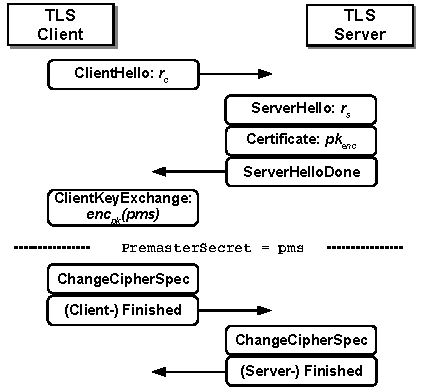
\includegraphics[width=\linewidth]{img/tls-handshake} 
	\caption{\textbf{TLS-RSA handshake.} After receiving an encrypted \pms, the server waits for an authenticated \texttt{ClientFinished} message.}
	\label{fig:tls-handshake}
\end{figure}
\fi

\paragraph{The TLS handshake protocol.}
In TLS~\cite{rfc5246} or \sslthree, the client initiates the handshake with a \texttt{ClientHello}, which contains a client random $r_c$ and a list of supported cipher suites. The server chooses one of the cipher suites and responds with three messages, \texttt{ServerHello}, \texttt{Certificate}, and \texttt{ServerHelloDone}. These messages include the server's choice of cipher suite, server nonce $r_s$, and a server certificate with an RSA public key. The client then uses the public key to encrypt a newly generated 48-byte \pms $pms$ and sends it to the server in a \texttt{ClientKeyExchange} message. The client and server then derive encryption and MAC keys from the \pms and the client and server random nonces. The details of this derivation are not important to our attack.  The client then sends \texttt{ChangeCipherSpec} and \texttt{Finished} messages. The \texttt{Finished} message authenticates all previous handshake messages using the derived keys. The server responds with its own \texttt{ChangeCipherSpec} and \texttt{Finished} messages.

The two main details relevant to our attacks are:
\begin{itemize}
	\item The \pms is always 48 bytes long, independent of the chosen cipher suite.  This is also true for export cipher suites.
	\item After receiving the \texttt{ClientKeyExchange} message, the server waits for the \texttt{ClientFinished} message, in order to authenticate the client.
\end{itemize}


\ifsubmit\relax\else
\subsubsection{Real-world protocol support}
TLSv1.0 is the most commonly supported protocol version, according to several surveys.  The SSL Labs SSL Pulse survey~\cite{ssllabs} reports that 98.6\% of about 140,000 popular TLS/SSL-enabled web sites supported TLSv1.0 in January 2016.  72.0\% supported TLSv1.2.  Support for \ssltwo was at 9.3\%, and \sslthree was at 29\%. Mayer et al.~\cite{DBLP:journals/corr/MayerZSH15} performed Internet-wide surveys of SMTP, IMAP, and POP3 between April and August 2015, and found that support for \ssltwo support was as high as 41.7\% of servers for SMTP on port 25 and as low as 3.7\% of IMAP servers on port 143.  Support for TLSv1.0 was nearly universal on these ports, varying from 91.6\% on port 25 to 98.9\% on port 143.

Bowen~\cite{bowencab} collected 213 million SSL/TLS client hellos and user agent strings from connections to popular sites, of which 183,000 (0.09\%) client hellos supported \ssltwo.  All of these client hellos also supported at least TLSv1.0.

Holz et al.~\cite{2016holz_analysis_tls-based_protocols_electronic_communication} performed passive monitoring to collect information about 16 million SSL/TLS connections during one week in July-August 2015.  They did not report any numbers for \ssltwo, and stated in personal communication that they did not observe any \ssltwo connections in their dataset.
\fi

%In response to our disclosure, OpenSSL has disabled \ssltwo by default in the 1.0.1r and 1.0.2f releases~\cite{opensslchangelog}.  

%This bug was also fixed in the aforementioned openssl releases.

\paragraph{OpenSSL SSLv2 cipher suite selection bug.}
\label{sec:openssl-selection}

We discovered that OpenSSL servers do not respect the cipher suites advertised
in the \ssltwo \texttt{ServerHello} message. That is, a malicious client can
select an \textit{arbitrary} cipher suite in the \texttt{ClientMasterKey}
message, regardless of the contents of the \texttt{ServerHello}, and force the
use of export cipher suites even if they are explicitly disabled in the server
configuration.  To fully detect \ssltwo oracles, we configured our scanner to
ignore the \texttt{ServerHello} cipher list. The cipher selection bug helps
explain the wide support for \ssltwo---the protocol appeared disabled, but 
non-standard clients could still complete handshakes.

%(this was not necessarily the case when OpenSSL was used as a plugin in Apache or other webservers).
%In addition to verifying this vulnerability in our lab, we have encountered several SSLv2 servers on the Internet which have apparently disabled export cipher suites (as judged by their \texttt{ServerHello} message), where we could indeed force the use of these cipher suites on those servers.

%In addition, these versions by default disabled \ssltwo support.

%\todo{Mention POP3 is likely vulnerable without any active attacks involving the client, since we expect to have a handshake every few minutes anyway}


\subsection{Bleichenbacher's attack}
\label{sec:bleichenbacher}
Bleichenbacher's attack is a padding oracle attack---it exploits the
fact that RSA ciphertexts should decrypt to plaintexts compliant with
the \PKCS padding format. If an implementation receives an RSA
ciphertext that decrypts to an invalid \PKCS plaintext, it might
naturally leak this information via an error message, by closing the
connection, or by taking longer to process the error condition.  This
behavior can leak information about the plaintext that can be modeled
as a cryptographic \textit{oracle} for the decryption
process. Bleichenbacher~\cite{Bleichenbacher} demonstrated how such an
oracle could be exploited to decrypt RSA ciphertexts.

%For example, the decrypting code may require different processing times for valid vs.\ invalid plaintexts - this is termed a "timing side-channel vulnerability". As another example, the decrypting code may send messages derived in some way from the plaintexts - this is termed a "direct message side channel vulnerability".
%The seminal work in this area \cite{Bleichenbacher} identified the general potential for such vulnerabilities, specifically using a direct message side channel vulnerability present in TLS implementations at the time, and demonstrated how such information could be gradually combined to eventually decrypt the RSA ciphertext in full.

\paragraph{Algorithm.}
In the simplest attack scenario, the attacker has a valid \PKCS
ciphertext $c_{0}$ that he wishes to decrypt to discover the message
$m_{0}$.  He has no access to the private RSA key, but instead has
access to an oracle $\Oracle$ that will decrypt a ciphertext $c$ and
inform the attacker whether the most significant two bytes match
the required value for a correct \PKCS padding:
\begin{equation*} 
\Oracle(c) =  
\begin{cases} 
1 & \text{ if } m=c^d \bmod N \text{ starts with \hexb{00}{02}} \\ 
0 & \text{ otherwise.} 
\end{cases} 
\end{equation*} 

If the oracle answers with \texttt{1}, the attacker knows that $2B
\leq m \leq 3B-1$, where $B = 2^{8(\ell-2)}$.  The attacker can take
advantage of RSA malleability to generate new candidate ciphertexts
for any $s$:
\[ 
c = (c_{0} \cdot s^e) \bmod N = (m_{0} \cdot s)^e \bmod N 
\] 
The attacker queries the oracle with $c$. If the oracle responds with
$0$, the attacker increments $s$ and repeats the previous
step. Otherwise, the attacker learns that for some~$r$, $2B \leq m_{0}s - rN  < 3B$. This allows the attacker to reduce the range of possible solutions to  
\[ 
\frac{2B+rN}{s} \leq m_{0} < \frac{3B+rN}{s}  
\] 
The attacker proceeds by refining guesses for $s$ and $r$ values and
successively decreasing the size of the interval containing $m_{0}$.  At
some point the interval will contain a single valid value, $m_{0}$.
Bleichenbacher's original paper describes this process in further
detail~\cite{Bleichenbacher}.

\paragraph{Countermeasures.}
In order to protect against this attack, the decrypter must not leak
any information about the \PKCS validity of the ciphertext.  Since the
ciphertext itself does not decrypt to a valid message, the
decrypter needs to generate a fake plaintext and continue with the
protocol using this decoy.  The attacker should not be able to
distinguish the resulting computation from a correctly decrypted
ciphertext.

In the case of SSL/TLS, the server generates a random \pms and finishes
the handshake with this random \pms if the decrypted ciphertext is
invalid.  The client will not possess the session key to send a valid
\texttt{ClientFinished} message and the connection will terminate.

